%%%%%%%%%%%%%%%%%%%%%%%%%%%%%%%%%%%%%%%%%
% Beamer Presentation
% LaTeX Template
% Version 1.0 (10/11/12)
%
% This template has been downloaded from:
% http://www.LaTeXTemplates.com
%
% License:
% CC BY-NC-SA 3.0 (http://creativecommons.org/licenses/by-nc-sa/3.0/)
%
%%%%%%%%%%%%%%%%%%%%%%%%%%%%%%%%%%%%%%%%%

%----------------------------------------------------------------------------------------
%	PACKAGES AND THEMES
%----------------------------------------------------------------------------------------

\documentclass[aspectratio=169]{beamer}

\mode<presentation> {

% The Beamer class comes with a number of default slide themes
% which change the colors and layouts of slides. Below this is a list
% of all the themes, uncomment each in turn to see what they look like.

%\usetheme{default}
%\usetheme{AnnArbor}
%\usetheme{Antibes}
%\usetheme{Bergen}
%\usetheme{Berkeley}
%\usetheme{Berlin}
%\usetheme{Boadilla}
%\usetheme{CambridgeUS}
%\usetheme{Copenhagen}
%\usetheme{Darmstadt}
%\usetheme{Dresden}
%\usetheme{Frankfurt}
%\usetheme{Goettingen}
%\usetheme{Hannover}
%\usetheme{Ilmenau}
%\usetheme{JuanLesPins}
%\usetheme{Luebeck}
\usetheme{Madrid}
%\usetheme{Malmoe}
%\usetheme{Marburg}
%\usetheme{Montpellier}
%\usetheme{PaloAlto}
%\usetheme{Pittsburgh}
%\usetheme{Rochester}
%\usetheme{Singapore}
%\usetheme{Szeged}
%\usetheme{Warsaw}

% As well as themes, the Beamer class has a number of color themes
% for any slide theme. Uncomment each of these in turn to see how it
% changes the colors of your current slide theme.

%\usecolortheme{albatross}
\usecolortheme{beaver}
%\usecolortheme{beetle}
%\usecolortheme{crane}
%\usecolortheme{dolphin}
%\usecolortheme{dove}
%\usecolortheme{fly}
%\usecolortheme{lily}
%\usecolortheme{orchid}
%\usecolortheme{rose}
%\usecolortheme{seagull}
%\usecolortheme{seahorse}
%\usecolortheme{whale}
%\usecolortheme{wolverine}

%\setbeamertemplate{footline} % To remove the footer line in all slides uncomment this line
%\setbeamertemplate{footline}[page number] % To replace the footer line in all slides with a simple slide count uncomment this line

%\setbeamertemplate{navigation symbols}{} % To remove the navigation symbols from the bottom of all slides uncomment this line
}

\usepackage{graphicx} % Allows including images
\usepackage{booktabs} % Allows the use of \toprule, \midrule and \bottomrule in tables

\usepackage{tikz}
\usetikzlibrary{arrows,shapes,positioning,shadows,trees,mindmap,calc}
\usepackage[absolute,overlay]{textpos}
  \setlength{\TPHorizModule}{1mm}
  \setlength{\TPVertModule}{1mm}

\addtobeamertemplate{frametitle}{}{%
\begin{textblock*}{100mm}(.85\textwidth,-0.25cm)
\includegraphics[scale=0.25]{logo.png}
\end{textblock*}}

%----------------------------------------------------------------------------------------
%	GRAPHICS PATH
%----------------------------------------------------------------------------------------
\graphicspath{{./fig/}}

%----------------------------------------------------------------------------------------
%	TITLE PAGE
%----------------------------------------------------------------------------------------

\title[PRT551 - Lecture 1]{Project Management, Risk, and Reliability} % The short title appears at the bottom of every slide, the full title is only on the title page

\author{Associate Professor Sureshkumar} % Your name
\institute[CDU] % Your institution as it will appear on the bottom of every slide, may be shorthand to save space
{
Charles Darwin University \\ % Your institution for the title page
\medskip
\textit{cdux@cdu.edu.au} % Your email address
}
\date{\today} % Date, can be changed to a custom date

\begin{document}

\begin{frame}
\titlepage % Print the title page as the first slide
\begin{textblock}{20}(110,25)
      \includegraphics[scale=0.8]{logo_1.png}
\end{textblock}
\end{frame}

%\begin{frame}
%\frametitle{Overview} % Table of contents slide, %comment this block out to remove it
%\tableofcontents % Throughout your presentation, if %you choose to use \section{} and \subsection{} %commands, these will automatically be printed on %this slide as an overview of your presentation
%\end{frame}

%----------------------------------------------------------------------------------------
%	PRESENTATION SLIDES
%----------------------------------------------------------------------------------------

%------------------------------------------------
%\section{Section 1} % Sections can be created in order to organize your presentation into discrete blocks, all sections and subsections are automatically printed in the table of contents as an overview of the talk
%------------------------------------------------

%\subsection{Subsection} % A subsection can be created just before a set of slides with a common theme to further break down your presentation into chunks

%------------------------------------------------
% Slide about introduction to course
\begin{frame}
\frametitle{Administration}
\textbf{What is this course on CDUX?}
\begin{itemize}
\item This course has been designed to give you a taste of Project Management, Risk and Reliability (PRT551) at Charles Darwin University;
\item This course is part of Charles Darwin University's Master of Engineering program;
\item The content delivered on this platform (CDUX) is the first 4 weeks of PRT551, which includes the first assignment for the course;
\item The assignment makes up 15\% of your grade for the course, and is credit eligible should you decide to continue your studies with Charles Darwin University 
\end{itemize}
\end{frame}

%------------------------------------------------
\begin{frame}
\frametitle{Administration}
\textbf{How should you study this course?}
\begin{itemize}
\item There are short 5 to 6 minute lectures which cover the intended learning outcomes each week.
\item Lecture slides are provided on the home page of the course for each week - you should print these out and take notes along with each lecture to help learn the course material.
\item Each 5 to 6 minute lecture is punctuated by some short exercises. Studies show that students learn more effectively when they are actively engaging with the content - make sure you have a go at these exercises.
\item There are tutorial exercises at the end of each week which will further help you to master the intended learning outcomes, and build the skills you need to address the final assignment.
\end{itemize}
\end{frame}
%------------------------------------------------
% Slide about textbook used for the course
\begin{frame}
\frametitle{Textbook \& Dicussion Forum}

\begin{columns}
\column{0.45\textwidth}
\begin{figure}
\includegraphics[scale=0.3]{textbook}
\caption{The textbook which is prescribed for the course.}
\end{figure}
\column{0.5\textwidth}
\textbf{Discussion Forum}\\
\vspace{0.5cm} \small
To promote community learning there is a discussion forum on which you can interact with your peers. Use this to ask questions if you are stuck, however, please observe the following etiquette on the forum:
\begin{itemize}
\item Polite respectful discourse is a must - the forum will be monitored and any offending material will be removed.
\item You are encouraged to help each other on the forum, but please do not post answers to the questions or tutorial questions. 
\end{itemize}
\end{columns}

\end{frame}

%------------------------------------------------
% Slide about learning objectives
\begin{frame}
\frametitle{Learning Objectives}
The learning objectives for this week are:\\

\begin{itemize}
\item Understand the growing need for better project, program, and portfolio management.
\item Explain what a \textbf{project} is, provide examples of projects, list various \textbf{attributes of projects}, and discuss the \textbf{triple constraints} of project management.
\item Describe \textbf{project management} and key elements of the \textbf{project management framework}, including project \textbf{stakeholders}, \textbf{project management knowledge areas}, \textbf{common tools and techniques}, and \textbf{project success factors}.
\item Discuss the relationship between project, program, and portfolio management and their contribution to enterprise success.
\item Describe the project management profession.
\end{itemize}
\end{frame}

%------------------------------------------------
% Slide about introduction to project management
\begin{frame}[fragile]
\frametitle{Introduction}
\begin{columns}
\column{0.45\textwidth}
\begin{figure}
\frame{\includegraphics[scale=0.25]{intro_1}}
\caption{The demand for the project management skill set is growing.}
\end{figure}
\vspace{-0.8cm}
\begin{figure}
\frame{\includegraphics[scale=0.25]{pm_jobs}}
\caption{Many countries have a large number of projected opportunities for growth in the project management profession.}
\end{figure}
\column{0.5\textwidth}
\begin{figure}
\frame{\includegraphics[scale=0.3]{pmbok_guide}}
\caption{The PMBOK is an authoritative guide to the project management profession, and this course will make reference to it frequently.}
\end{figure}
\vspace{-0.5cm}
\tiny (Source: http://www.pmi.org/-/media/pmi/documents/public/pdf/business-solutions/project-management-skills-gap-report.pdf)
\end{columns}
\end{frame}

%------------------------------------------------
% Slide: what is a project?
\begin{frame}
\frametitle{What is a project?}
Business activities can be roughly categorised into the following 2 categories:
\begin{figure}
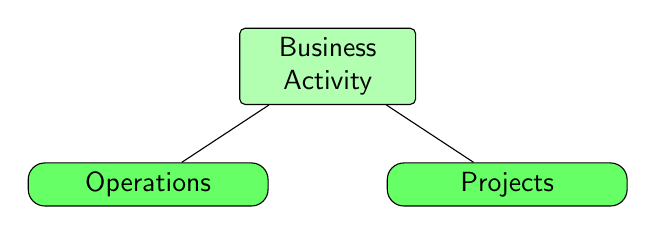
\begin{tikzpicture}
\tikzset{
  basic/.style  = {draw, text width=2cm, font=\sffamily, rectangle},
  root/.style   = {basic, rounded corners=2pt, thin, align=center,
                   fill=green!30},
  level 2/.style = {basic, rounded corners=6pt, thin,align=center, fill=green!60,
                   text width=8em},
  level 3/.style = {basic, thin, align=left, fill=pink!60, text width=6.5em}
}

level 1/.style={sibling distance=40mm},
  edge from parent/.style={->,draw},
  >=latex]
  
\node[root] {Business Activity}
% The first level, as children of the initial tree
  child {node[level 2, left] (c1) {Operations}}
  child {node[level 2, right] (c2) {Projects}};
\end{tikzpicture}
\end{figure}

\begin{block}{Definition: \textbf{Project}}
A \textbf{project} is a temporary endeavour undertaken to create a unique product, service, or result.
\end{block}
\begin{block}{Definition: \textbf{Operation}}
An \textbf{operation} is on-going work done in an organisation to sustain the business.
\end{block}
\end{frame}

%------------------------------------------------
% Slide: project attributes
\begin{frame}
\frametitle{Project Attributes}
A \textbf{project} is distinguished by a number of attributes, most notably a project:
\begin{itemize}
\item has a unique purpose;
\item is temporary;
\item is developed using progressive elaboration or in an iterative fashion;
\item requires resources, often from various areas;
\item should have a primary customer or sponsor (the project sponsor usually provides the direction and funding for the project)
\item involves uncertainty
\end{itemize} 
\end{frame}

%------------------------------------------------
\begin{frame}
\frametitle{Project Success}
There are different ways to define project success. Some of them include:
\begin{itemize}
\item The project satisfied the customer/sponsor.
\item The project met all of the desired results.
\item The project achieved the desired outcomes and met \textbf{scope}, \textbf{time}, and \textbf{cost} constraints. 
\end{itemize}
\end{frame}

%------------------------------------------------
\begin{frame}
\frametitle{Project Constraints}
\begin{columns}
\column{0.45\textwidth} \small
Every project is constrained in different ways, however, many project managers choose to focus on three simple categories (often called the \textbf{triple constraints}):
\begin{itemize} \small
\item \textbf{Scope}: is the work that will be done as part of the project. More specifically, it is the product, service, or result that the customer or sponsor expects from completion of the project.
\item \textbf{Time}: is the time it should take to complete the project, and the project's schedule.
\item \textbf{Cost}: is the costs involved with completing the project.
\end{itemize}
\column{0.5\textwidth}
\begin{figure}
\scalebox{0.4}{
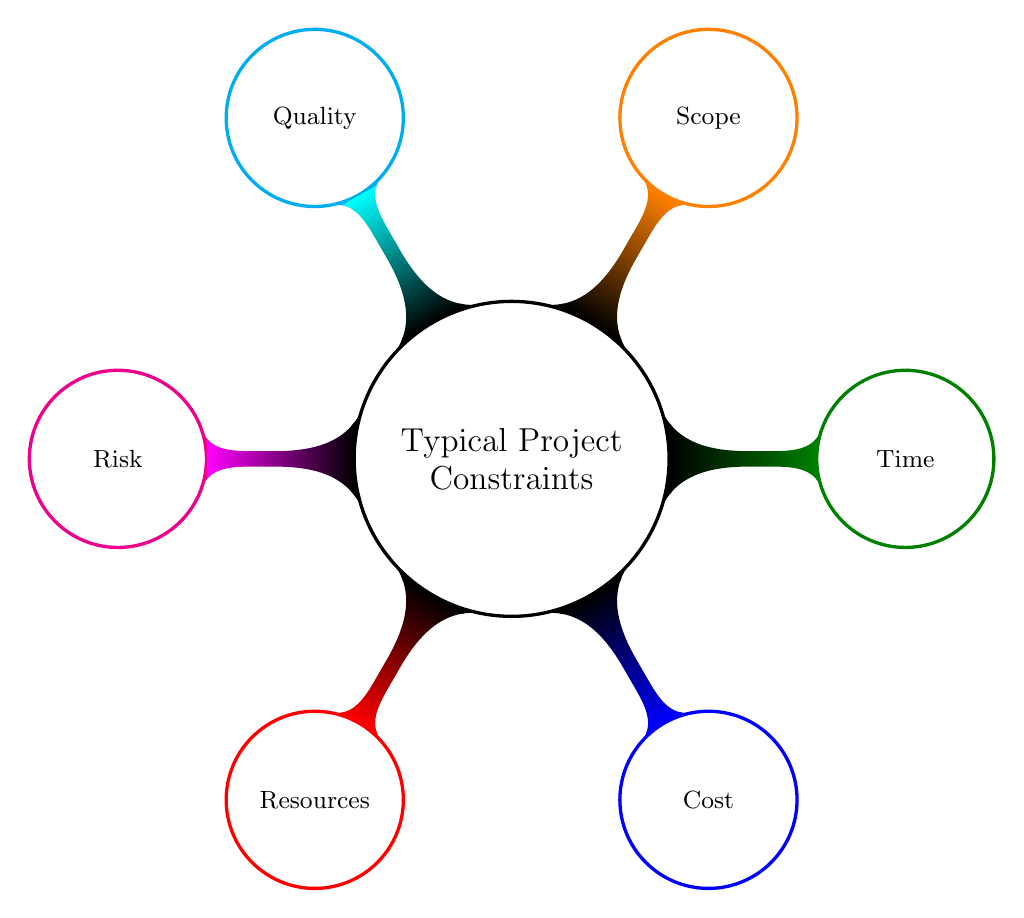
\begin{tikzpicture}
  \tikzset{concept/.append style={fill={none}}}
  \path[mindmap,concept color=black,text=black]
    node[concept] {Typical Project Constraints}
    [clockwise from=0]
    child[concept color=green!50!black] {node[concept] {Time}}  
    child[concept color=blue] {node[concept] {Cost}}
    child[concept color=red] {node[concept] {Resources} }
    child[concept color=magenta] { node[concept] {Risk} }
    child[concept color=cyan] { node[concept] {Quality} }
    child[concept color=orange] { node[concept] {Scope} };
\end{tikzpicture}
}
\caption{There are other constraints that are considered also, shown in the figure above.}
\end{figure}
\end{columns}
\end{frame}

%------------------------------------------------
\begin{frame}
\frametitle{A Handy Mathematical Analogy}
Suppose $\textbf{x}$ is a vector of inputs to the project that a project manager can control. It can be useful to think of a project as the following optimisation problem:
\begin{equation*}
\begin{matrix}
\displaystyle \max_{\textbf{x}} & f_{\textrm{success}}(\textbf{x})  \\
\textrm{s.t.} & \textrm{scope}(\textbf{x}) \\
& \textrm{time}(\textbf{x}) \\
& \textrm{cost}(\textbf{x})
\end{matrix}
\end{equation*}
\end{frame}

%------------------------------------------------
\begin{frame}
\frametitle{What is Project Management?}
\begin{block}{Definition: \textbf{Project Management}}
\textbf{Project management} is the application of knowledge, skills, tools, and techniques to project activities to meet project requirements.
\end{block}
\end{frame}

%------------------------------------------------
\begin{frame}
\frametitle{Project Management Framework}
The project management framework can be broken down in two ways: by \textbf{Process Groups}, or by \textbf{Knowledge Areas}. There are 5 different \textbf{process groups}, and 10 different \textbf{knowledge areas}.
\vspace{-0.5cm}
\begin{columns}[t]
\column{0.45\textwidth}
\begin{block}{Definition: \textbf{Process Groups}}
\begin{enumerate} \footnotesize
\item Initiating
\item Planning
\item Executing
\item Monitoring and controlling
\item Closing
\end{enumerate}
\end{block}
\column{0.45\textwidth}
\begin{block}{Definition: \textbf{Knowledge Areas}}
\begin{enumerate} \footnotesize
\item Integration
\item Scope
\item Time
\item Cost
\item Quality
\item Human resource
\item Communication
\item Risk
\item Procurement
\item Stakeholder management
\end{enumerate}
\end{block}
\end{columns}
\end{frame}

%------------------------------------------------
\begin{frame}
\frametitle{Project Management Framework}
\begin{figure}
\includegraphics[scale=0.3]{mapping}
\end{figure}
\end{frame}

%------------------------------------------------
\begin{frame}
\frametitle{Five Areas of Expertise}
To undertake any project you need human labour. Different people have different skill sets. The project management framework categorises these skills into 5 main categories:
\vspace{0.5cm}
\begin{block}{Definition: \textbf{Areas of Expertise}}
\begin{enumerate}
\item PMBOK
\item Area knowledge, standards, and regulations
\item Project Environment
\item Management skills
\item Interpersonal skills
\end{enumerate}
\end{block}
\end{frame}

%------------------------------------------------
\begin{frame}
\frametitle{Five Areas of Expertise}
\begin{figure}
\scalebox{0.8}{
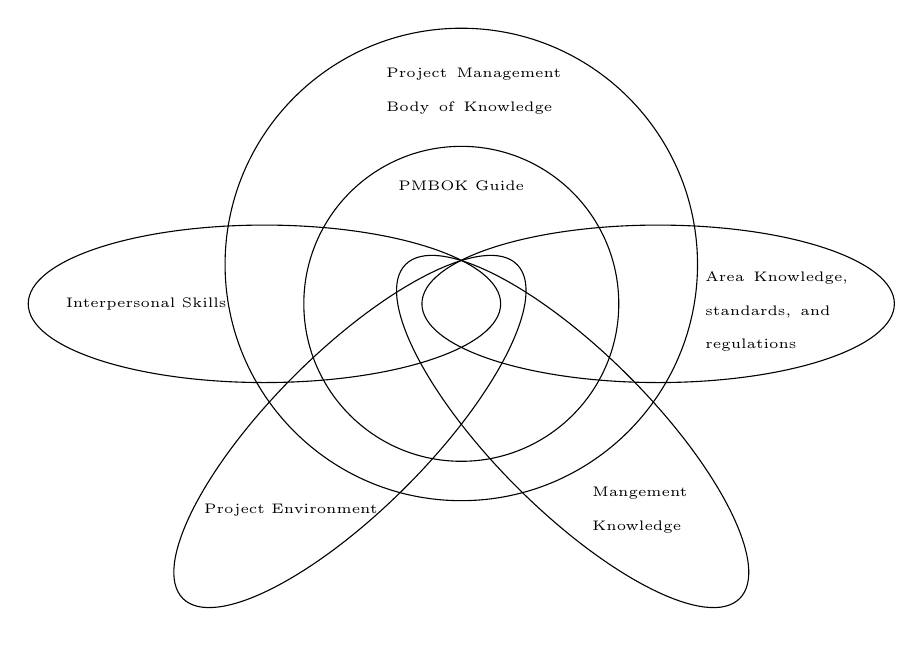
\begin{tikzpicture}
\draw (0,0) circle (3cm) node [xshift=0.3cm,yshift=2.2cm, text width=2.5cm] {\tiny Project Management Body of Knowledge};
\draw (0,-0.5) circle (2cm) node [yshift=1.5cm] {\tiny PMBOK Guide};
\draw (-2.5,-0.5) ellipse (3cm and 1cm) node [xshift=-1.5cm] {\tiny Interpersonal Skills};
\draw (2.5,-0.5) ellipse (3cm and 1cm) node [xshift=1.6cm, yshift=-0.1cm,text width=2cm] {\tiny Area Knowledge, standards, and regulations};
\draw[cm={cos(45) ,-sin(45) ,sin(45) ,cos(45) ,(0,0)}] (2.5,-0.5) ellipse (3cm and 1cm) node [xshift=1cm,yshift=-1cm,text width=1.5cm] {\tiny Mangement Knowledge};
\draw[cm={cos(-45) ,-sin(-45) ,sin(-45) ,cos(-45) ,(0,0)}] (-2.5,-0.5) ellipse (3cm and 1cm) node [xshift=-0.75cm,yshift=-1cm] {\tiny Project Environment};
\end{tikzpicture}
}
\end{figure}
\end{frame}

%------------------------------------------------
\begin{frame}
\frametitle{Five Areas of Experise}
\textbf{Application area knowledge, standards, and regulations}\\
\vspace{0.5cm}
This area of expertise can be broken down into the following sub-categories:
\begin{itemize}
\item Functional - legal, marketing
\item Technical - software, engineering
\item Management Specialisation - government, community, development
\item Industry Groups - automotive, finance
\end{itemize}
\begin{block}{International Organisation Standardisation (ISO)}
Standards - established by concensus\\
Regulation - government imposed
\end{block}
\end{frame}

%------------------------------------------------
\begin{frame}
\frametitle{Five Areas of Experise}
\textbf{Project Environment}\\
\vspace{0.5cm}
\begin{columns}
\column{0.45\textwidth}
\begin{itemize}
\item Cultural and social environment
\item International and political environment
\item Physical environment
\end{itemize}
\column{0.5\textwidth}
\begin{figure}
\frame{\includegraphics[scale=0.4]{handshake}}
\end{figure}
\end{columns}
\end{frame}

%------------------------------------------------
\begin{frame}
\frametitle{Five Areas of Experise}
\textbf{Management Knowledge and Skills}\\
\vspace{0.5cm}
\begin{columns}[b]
\column{0.45\textwidth}
\begin{figure}
\includegraphics[scale=0.23]{management}
\end{figure}
\column{0.5\textwidth}
\begin{itemize}
\item Planning
\item Organising
\item Staffing
\item Executing
\item Controlling operations
\end{itemize}
\end{columns}
\end{frame}

%------------------------------------------------
\begin{frame}
\frametitle{Five Areas of Experise}
\textbf{Interpersonal Skills}\\
\vspace{0.5cm}
\begin{columns}[t]
\column{0.45\textwidth}
\begin{itemize}
\item Effective communication
\item Influencing organisation - getting things done
\item Leadership - vision and strategy
\item Motivation - energise, overcome obstacles
\item Negotiation and conflict management
\item Problem solving
\end{itemize}

\column{0.5\textwidth}
\begin{figure}
\frame{\includegraphics[scale=0.3]{interpersonal_skills}}
\end{figure}
\end{columns}
\end{frame}

%------------------------------------------------
\begin{frame}
\frametitle{Project Life Cycle}
\begin{figure}
\frame{\includegraphics[scale=0.4]{project_life_cycle}}
\caption{Graph shows how cost, uncertainty, cost of change, and influence of stakeholders changes over the project life cycle.}
\end{figure}
\end{frame}

%------------------------------------------------
\begin{frame}
\frametitle{Project Phases}
Often, especially for larger projects which have extended duration, it is useful to break the project up into phases. Typically, the completion of one or more deliverables signifies a project phase.
\vspace{0.5cm}
\begin{block}{Definition: \textbf{Deliverable}}
A \textbf{deliverable} is defined as a measurable, verifiable work product. Some examples include:
\begin{itemize}
\item Specification
\item Feasibility study
\item Design document
\item Prototype
\end{itemize}
\end{block}
\end{frame}

%------------------------------------------------
\begin{frame}
\frametitle{Project Stakeholders}
\begin{block}{Definition: \textbf{Stakeholders}}
\textbf{Stakeholders} are the individuals and/or organisations that are actively involved in the project, or whose interests may be affected as a result of project execution or project completion.
\end{block}
\vspace{0.5cm}
\begin{columns}
\column{0.45\textwidth}
Some examples of stakeholders include:
\begin{itemize}
\item The project sponsor
\item The project manager
\item The project team
\item Support staff
\item Customers
\item Suppliers
\item Opponents to the project
\end{itemize}
\column{0.5\textwidth}
Anybody affected by the planned project can constitute as a stakeholder - it's just the level of influence that is relevant.
\end{columns}
\end{frame}

%------------------------------------------------
\begin{frame}
\frametitle{Project Stakeholders}
\begin{block}{Definition: Positive Stakeholder}
A \textbf{positive stakeholder} is a stakeholder which benefits from the project's success
\end{block}
\vspace{0.5cm}
\begin{block}{Definition: Negative Stakeholder}
A \textbf{negative stakeholder} is a stakeholder which is disadvantaged by the project's success.
\end{block}
\end{frame}

%------------------------------------------------
\begin{frame}
\frametitle{Organisational Influences}
Organisational culture has a direct influence on the project, for example:
\begin{itemize}
\item An aggressively entrepreneurial environment my be conducive to high-risk projects.
\item An authoritarian environment may not be conducive to participative approaches.
\end{itemize}
\end{frame}

%------------------------------------------------
\begin{frame}
\frametitle{What is a Program?}
\begin{block}{Definition: \textbf{Program}}
A \textbf{program} is a group of related projects managed ina coordinated way to obtain benefits and control not available from managing them individually.
\end{block}
\vspace{0.5cm}
\begin{block}{Definition: \textbf{Program Manager}}
A \textbf{program manager} provides leadership and direction for the project managers heading the projects within the program.
\end{block}
\begin{figure}
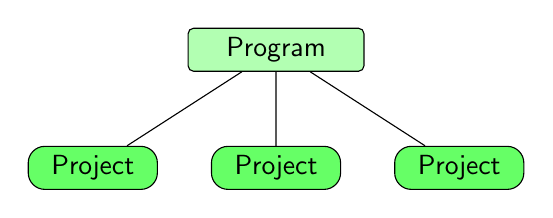
\begin{tikzpicture}
	\tikzset{
	  basic/.style  = {draw, text width=2cm, font=\sffamily, rectangle},
	  root/.style   = {basic, rounded corners=2pt, thin, align=center,
	                   fill=green!30},
	  level 2/.style = {basic, rounded corners=6pt, thin,align=center, fill=green!60,
	                   text width=4em},
	  level 3/.style = {basic, thin, align=left, fill=pink!60, text width=6.5em}
	}
	
	level 1/.style={sibling distance=40mm},
	  edge from parent/.style={->,draw},
	  >=latex]
	  
	\node[root] {Program}
	% The first level, as children of the initial tree
	  child {node[level 2, left] (c1) {Project}}
	  child {node[level 2] (c2) {Project}}
	  child {node[level 2, right] (c3) {Project}};
\end{tikzpicture}
\end{figure}
\end{frame}

%------------------------------------------------
\begin{frame}
\frametitle{Project Portfolio Management}
\begin{block}{Definition: \textbf{Project Portfolio Management}}
\textbf{Project portfolio management} is an emerging business strategy in which organisations group and manage projects and programs as a portfolio of investments that contribute to the entire enterprise's success.
\end{block}
\vspace{0.5cm}
\begin{figure}
\tikzset{
	  basic/.style  = {draw, text width=2cm, font=\sffamily, rectangle},
	  root/.style   = {basic, rounded corners=2pt, thin, align=center,
	                   fill=green!30},
	  level 2/.style = {sibling distance=40mm, basic, rounded corners=6pt, thin,align=center, fill=green!60,
	                   text width=4em},
	  level 3/.style = {sibling distance=40mm, basic, thin, align=left, fill=pink!60, text width=6.5em}
	}
\begin{tikzpicture}[
	level 1/.style={sibling distance=20mm},
	  edge from parent/.style={->,draw},
	  >=latex]
	  
	\node[root] {Portfolio}
	% The first level, as children of the initial tree
	  child {node[level 2, left] (c1) {Project}}
	  child {node[level 2] (c2) {Program}}
	  child {node[level 2] (c3) {Project}}
	  child {node[level 2, right] (c4) {Program}};
\end{tikzpicture}
\end{figure}
\end{frame}

%------------------------------------------------
\begin{frame}
\frametitle{\large Project Management Compared to Portfolio Management}
\begin{figure}
\includegraphics[scale=0.5]{program_mgt}
\caption{The figure shows the differences between project management and program management.}
\end{figure}
\end{frame}
%------------------------------------------------
\begin{frame}
\begin{center}
\huge The End
\end{center}
\end{frame}
\end{document} 